\documentclass[11pt,a4paper]{article}

% Packages
\usepackage[utf8]{inputenc}
\usepackage[spanish, es-tabla]{babel}
\usepackage{caption}
\usepackage{listings}
\usepackage{adjustbox}
\usepackage{enumitem}
\usepackage{boldline}
\usepackage{amssymb, amsmath}
\usepackage[margin=1in]{geometry}
\usepackage{xcolor}
%\usepackage{soul}
\usepackage{enumerate}
\usepackage{graphics, graphicx, float}

% Meta
\title{Guión de desactivación de bombas.}
\author{Estructura de Computadores - Práctica 3}
\date{José Antonio Álvarez Ocete}

% Custom
\providecommand{\abs}[1]{\lvert#1\rvert}
\setlength\parindent{0pt}
\definecolor{Light}{gray}{.90}
\newcommand\ddfrac[2]{\frac{\displaystyle #1}{\displaystyle #2}}

\begin{document}
\maketitle 

Las herramientas utilizadas en esta práctica para la desactivación de las distintas bombas serán gdb, ghex, objdump y strings. \\

\title{\large{\textbf{\underline{Bomba de prueba.}}}} \\

\textbf{En primer lugar, ejecutaremos la bomba sin que esta explote.} Para ello localizaremos los puntos clave en el código que hacen que la bomba explote. Ejecutamos 'gdb bomb' y colocamos un breakpoint al inicio del main con 'break main'. Por otro lado, ejecutamos 'objdump -D bomba $>>$ bomba.dump' y abrimos este archivo con un editor de texto para que nos sea más cómodo. \\

El proceso a seguir a continuación es el siguiente, ejecutaremos el programa con gdb mediante 'rnu' e iremos ejecutando instrucción a instrucción. Cuando la bomba explote, nos fijamos en el último salto realizado y colocamos un breakpoint en la comprobación realizada con anterioridad (break *0x$<$dirección$>$). Cuando lleguemos en la ejecución a dicha direccion, cambiaremos los valores de los registros mediante 'set \$eax = n' o 'set \$eax = \$edx' de forma tal que pase la comprobación y no llama a la función de la explosión. \\ 

En este caso, podemos usar las siguientes instrucciones:
\begin{itemize}
	\item En el breakpoint 2: 'set \$eax = 0'. 
	\item En el breakpoint 3: 'set \$rax = 0'.
	\item En el breakpoint 4: 'set \$eax = \$edx'.
	\item En el breakpoint 5: 'set \$eax = 0'.
\end{itemize}

Tras este procedimiento, el programa termina con la bomba desactivada. \\

\begin{figure}[H] 
 \centering
 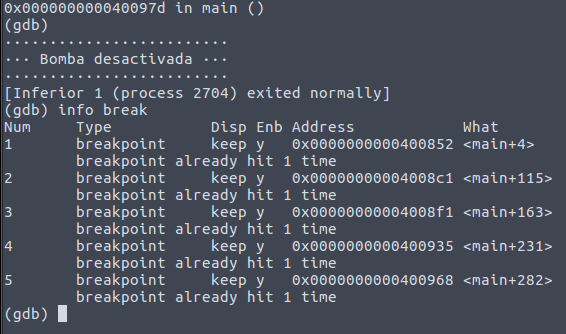
\includegraphics[scale=0.45]{capturas/prueba1.png} 
 \caption{Bomba de prueba - gdb} \label{fig:figura25}
\end{figure}

\textbf{A continuación, modificamos la bomba para que nunca explote.}  Para ello utilizamos el editor 'ghex' y las direcciones ya conocidas. Buscamos las direcciones en el desensamblado obtenido mediante objdump. Utilizaremos $"$Ctrl + F$"$ en el programa ghex, introduciendo el código en hexadecimal de la instrucción de salto (y de algunos valores adyacentes si obtenemos demasiados resultados) para encontrar dicha intrucción en el editor. Modificamos ahora el valor 74/7E (según la instrucción) por el valor EB, haciendo del salto uno de tipo incondicinal. Si repetimos esto para los 4 saltos (los 4 breakpoints del apartado anterior), la bomba no explotará cuando la volvamos a compilar y ejecutar. \\

\begin{figure}[H] 
 \centering
 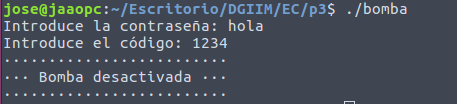
\includegraphics[scale=0.45]{capturas/prueba2.png} 
 \caption{Bomba de prueba modificada} \label{fig:figura25}
\end{figure}

\textbf{Por último, buscamos las claves de desactivación de la bomba.} Si miramos los valores con las que se realizan las comparaciones 2 y 4, nos daremos cuenta de que los valores máximos del tiempo que tenemos para introducir las claves son ambos 5 segundos. Por otro lado, $"$-$d"$, nos mostrará unicamente las strings del apartado $"$\emph{data}$"$ del gdb. \\

Si ejecutamos $"$\emph{strings -d bomba}$"$, el último valor de salida es abracadabra. Al probarla descubrimos que esta es efectivamente la contraseña. Por otro lado, si ejecutamos $"$\emph{strings bomba}$"$, la primera string después de \emph{main} es \emph{passcode}. Sería lógico que esta variable tuviese guardado el código, al ser la primera variable definida. Ejecutamos gdc sobre la bomba y $"$\emph{print passcode}$"$, obteniendo \emph{7777} que, con una rápida comprobación, confirmamos como código de nuestra bomba. \\

\begin{figure}[H] 
 \centering
 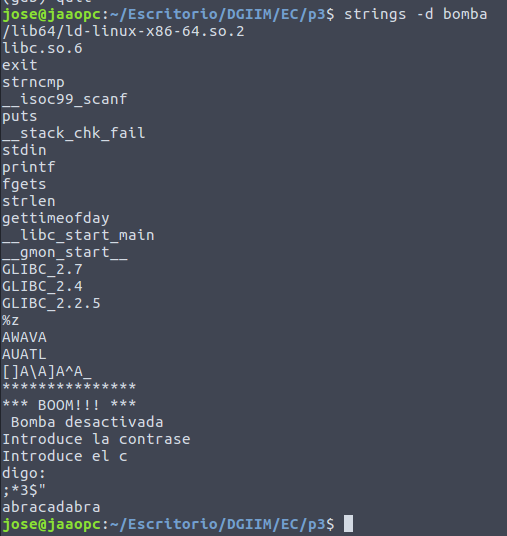
\includegraphics[scale=0.45]{capturas/prueba3.png} 
 \caption{Bomba de prueba - strings} \label{fig:figura25}
\end{figure}

\begin{figure}[H] 
 \centering
 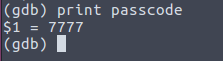
\includegraphics[scale=0.45]{capturas/prueba4.png} 
 \caption{Bomba de prueba - print} \label{fig:figura25}
\end{figure}

\begin{figure}[H] 
 \centering
 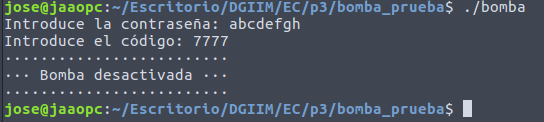
\includegraphics[scale=0.45]{capturas/prueba5.png} 
 \caption{Bomba de prueba resuelta} \label{fig:figura25}
\end{figure}

\title{\large{\textbf{\underline{Bomba 1: Bomba\_NBA\_2015}}}} \\

Lo primero que he hecho es ejecutar la bomba. Se nos pregunta un código y una contraseña. Después de introducir ambas, la bomba explota. Tras esta primera ejecución, probamos suerte con el comando strings. Para los datos globlaes (\emph{$"$strings Bomba\_NBA\_201$"$}) no obtengo nada en claro, pero cuando lo ejecutamos unicamente sobre el bloque \emph{data}: \\

\begin{figure}[H] 
	\centering
	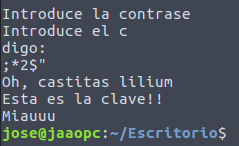
\includegraphics[scale=0.45]{capturas/nba1.png} 
	\caption{Bomba NBA - strings} \label{fig:figura25}
\end{figure}

Tras esta salida de datos, pensé que la clave era "Miauuu", y tras mucho tiempo buscando el cogio, terminé de entender el algoritmo del programa, y descubrí que la contraseña era "Oh, castitas lilium". En realidad, el programa realiza varias comprobaciones con otras claves posibles, pero solamente la combinación de dos de ellas hace que el valo final de una variable sea el esperado. \\

\textbf{En primer lugar, ejecutaremos la bomba sin que esta explote.} Para ello basta con ejecutar el código con ciertos breakpoints e ir cambiando el valor de ciertos registros:

\begin{itemize}
	\item Breakpoint 1 - 0x804881a - set \$eax = 0
	\item Breakpoint 2 - 0x8048850 - set \$eax = 0
	\item Breakpoint 3 - 0x8048885 - set \$eax = \$edx
	\item Breakpoint 4 - 0x80488c1 - set \$eax = 0
\end{itemize}

\begin{figure}[H] 
	\centering
	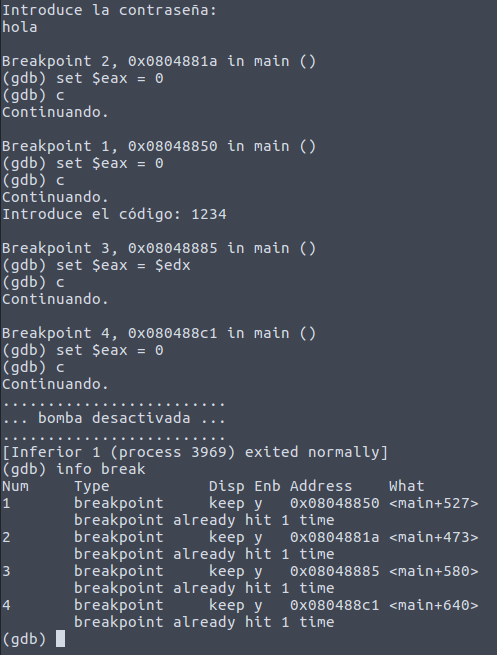
\includegraphics[scale=0.45]{capturas/nba2.png} 
	\caption{Bomba NBA gdb} \label{fig:figura25}
\end{figure}

\textbf{A continuación, modificamos la bomba para que nunca explote.}  Para ello utilizamos el editor 'ghex' y las direcciones ya conocidas, aplicaremos el mismo método que en la bomba de prueba, cambiando los saltos del apartado anterior a saltos incondicionales. Además, debemos cambiar el primer y el tercer salto de fomra que el valor del salto en si sea 0. Es decir, que en realidad no salte (de esta forma, se ejecutará siempre el código que está debajo). \\

\begin{figure}[H] 
	\centering
	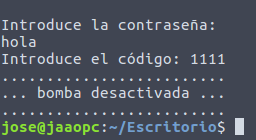
\includegraphics[scale=0.45]{capturas/nba3.png} 
	\caption{Bomba NBA modificada} \label{fig:figura25}
\end{figure}

\textbf{Por último, buscamos las claves de desactivación de la bomba.} Para ello usamos \emph{$"$strings -d Bomba\_NBA\_201$"$}, gdb y el comando \emph{x/20cb 0x$<$dirección$>$} en las direcciones donde se almacenan las claves. De esta forma llegamos a conocer las claves: \textbf{$"$Oh, castitas lilium$"$} y \textbf{$"$1030$"$}. \\


\begin{figure}[H] 
	\centering
	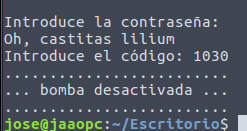
\includegraphics[scale=0.45]{capturas/nbaFIN.png} 
	\caption{Bomba NBA resuelta} \label{fig:figura25}
\end{figure}

\title{\large{\textbf{\underline{Bomba 2: bombaSofia}}}} \\

\textbf{En primer lugar, ejecutaremos la bomba sin que esta explote.} Para ello me remito al proceso utilizado en la bomba anterior, ejecutar el programa en gdb, colocando ciertos breakpoints y modificando los valores de los registros al alcanzarlos. Los breakpoints utilzados son:

\begin{itemize}
	\item Breakpoint 1 - 0x80486a5 - set \$eax = 0
	\item Breakpoint 2 - 0x80486d0 - set \$eax = 0
	\item Breakpoint 3 - 0x8048705 - set \$eax = \$edx
	\item Breakpoint 4 - 0x8048730 - set \$eax = 0
\end{itemize}

\begin{figure}[H] 
	\centering
	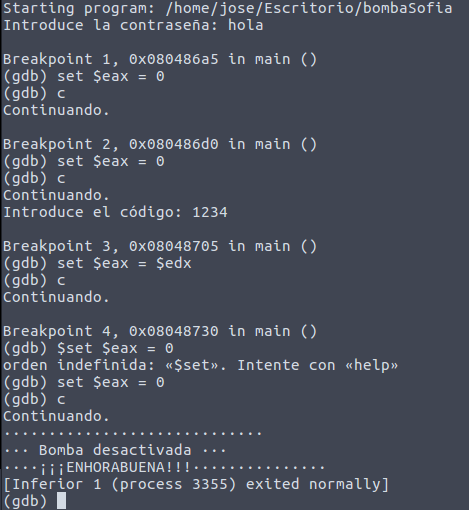
\includegraphics[scale=0.45]{capturas/bombasofia1.png} 
	\caption{Bomba Sofia - gdb} \label{fig:figura25}
\end{figure}

\textbf{A continuación, modificamos la bomba para que nunca explote.} De nuevo, acudimos a ghex para modificar el código. En esta bomba bastará con hacer todos los saltos incondicionales. \\

\begin{figure}[H] 
	\centering
	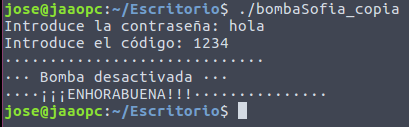
\includegraphics[scale=0.45]{capturas/bombasofia2.png} 
	\caption{Bomba Sofia modificada} \label{fig:figura25}
\end{figure}

\textbf{Por último, buscamos las claves de desactivación de la bomba.} En primer lugar, he usado el comando \emph{"strings"}, obteniendo una posible clave (\textbf{prohibidodesactivacio}), y lo que podría ser el nombre de la variable donde se alamacena la clave (\textbf{passcode}). Al introducir la contraseña, la bomba ha explotado, asi que he pensado que esta no era. 
Tras un vistazo al código, he ejecutado \emph{"x/20cb 0x804a030"}, obteniendo como salida la contraseña que ya tenía. He vuelto a introducir la clave pero más rápido, ya que era cuestión del tiempo, obteniendo como resultado que la contraseña era la ya obtenida. \\
Por otro lado, he ejecutado gdb y la instrucción \emph{"print passcode"}, obteniendo \textbf{4} como resultado. Ya tenemos nuestras claves: \textbf{prohibidodeactivacion} y \textbf{4}. \\

\begin{figure}[H] 
	\centering
	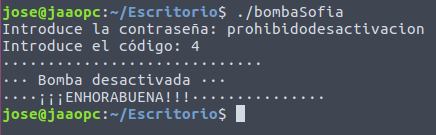
\includegraphics[scale=0.45]{capturas/bombasofia3.png} 
	\caption{Bomba Sofia resuelta} \label{fig:figura25}
\end{figure}

\title{\large{\textbf{\underline{Bomba 3: bomba\_antcc}}}} \\

La mayor cmoplejida que tiene esta bomba es donde guarda las contraseñas y el cambio de nombres de las funciones. La función en la que explota la bomba se llama \emph{gettimeofday\_plt}, distinta de la función que usamos para obtener el tiempo, \emph{gettimeofday@plt}, y la función para la desactivación de la bomba se llama \emph{booom}. Una vez descubierto este detalle, la bomba se hace más sencilla. \\

\textbf{En primer lugar, ejecutaremos la bomba sin que esta explote.} Repetimos el proceso de las bombas anteriores, esta vez 'esquivando' la llamadas a la función \emph{gettimeofday\_plt}. \\
La pista que podemos obtener es \emph{Look at the names}, que imagino que hace referencia a los nombres de las funciones. \\
Aquí están los breakpoints utilizados: \\

\begin{itemize}
	\item Breakpoint 1 - 0x8048785 - set \$eax = 0
	\item Breakpoint 2 - 0x80487ce - set \$eax = \$edx
	\item Breakpoint 3 - 0x80487fc - set \$eax = 0
	\item Breakpoint 4 - 0x8048814 - set \$eax = 0
	\item Breakpoint para obtener la pista - 0x804883b - set \$eax = 0x7e0
\end{itemize}

\begin{figure}[H] 
	\centering
	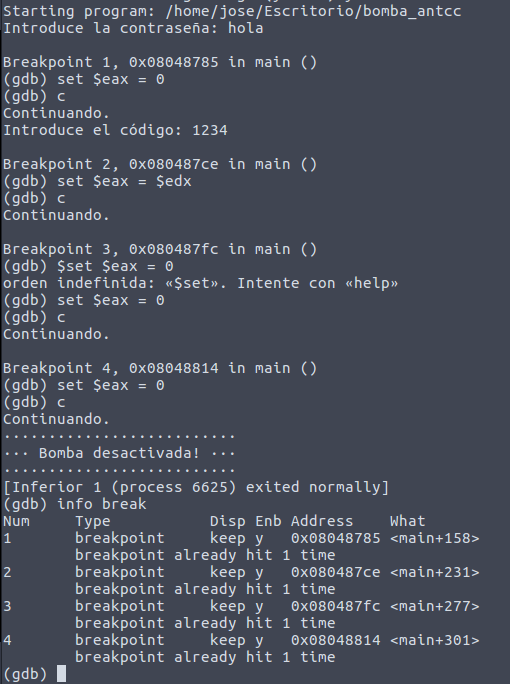
\includegraphics[scale=0.45]{capturas/antcc1.png} 
	\caption{Bomba Antcc - gdb} \label{fig:figura25}
\end{figure}

\textbf{A continuación, modificamos la bomba para que nunca explote.} De nuevo, acudimos a ghex para modificar el código. En esta bomba bastará con cambiar los saltos asociados a los primeros 4 breakpoints del apartado anterior. \\

\begin{figure}[H] 
	\centering
	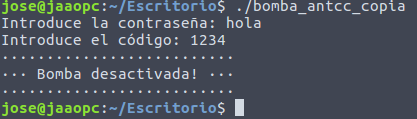
\includegraphics[scale=0.45]{capturas/antcc2.png} 
	\caption{Bomba Antcc modificada} \label{fig:figura25}
\end{figure}

\textbf{Por último, buscamos las claves de desactivación de la bomba.} En primer lugar, he usado el comando \emph{"strings"}, obteniendo tres posibles claves: \emph{Bolzano}, \emph{Weierstrasss} y \emph{Nadaaaaaaaaaa}. Además, al ejecutarlo con \emph{-d} he obtenido lo que podría ser el nombre de la variable donde se alamacena la clave (\emph{codigo}). 
Usando gdb, he hecho \emph{print codigo}, obteniendo n 4, que ha resultado no ser la contraseña. He depurado entonceshasta el segundo breakpoint y, en vez de ejecutar \emph{set \$eax = \$edx}, obteniendo así el código: \textbf{3584}. \\
Finalmente he introducido el código obtenido en combinación con las 3 contraseñas obtenidas mediante \emph{strings}, quedando desactivada la bomba con la segunda. Ya tenemos nuestras claves: \textbf{Weierstrasss} y \textbf{3584}. \\

\begin{figure}[H] 
	\centering
	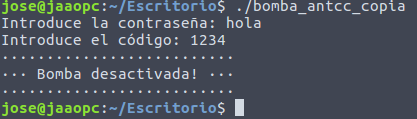
\includegraphics[scale=0.45]{capturas/antcc2.png} 
	\caption{Bomba Antcc resuelta} \label{fig:figura25}
\end{figure}

\title{\large{\textbf{\underline{Bomba 4: bcegarra}}}} \\

Tras realizar 5 bombas (esta es la última que he hecho, después de la mía), tengo cierta soltura en el proceso. He resuelto esta bomba mucho más rápido de lo que esperaba, aunque también era más sencilla de lo que creía. Procedamos a la desactivación. \\

\textbf{En primer lugar, ejecutaremos la bomba sin que esta explote.} Para ello he utilizado los siguientes breakpoints:

\begin{itemize}
	\item Breakpoint 1 - 0x8048729 - set \$eax = 0
	\item Breakpoint 2 - 0x8048752 - set \$eax = 0
	\item Breakpoint 3 - 0x80487b9 - set \$eax = 0
	\item Breakpoint 4 - 0x80488e2 - set \$eax = 0
\end{itemize}

\begin{figure}[H] 
	\centering
	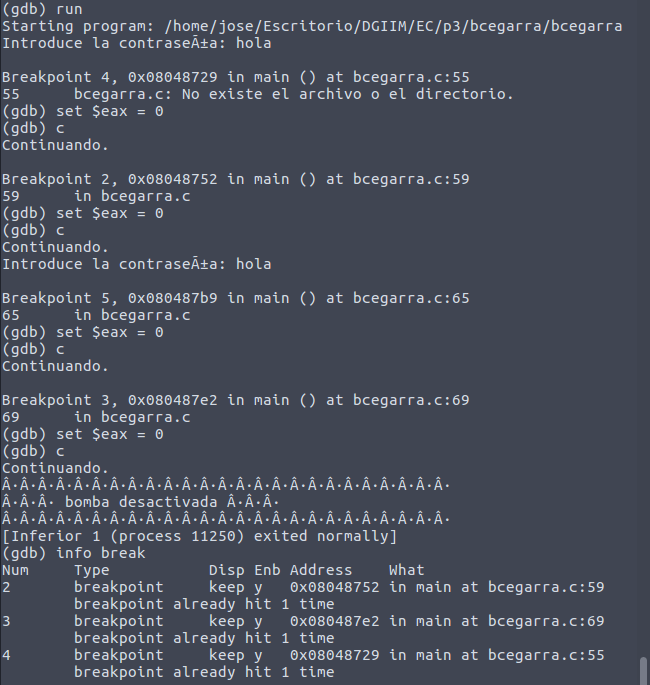
\includegraphics[scale=0.45]{capturas/bcegarra1.png} 
	\caption{Bomba Bcegarra - gdb} \label{fig:figura25}
\end{figure}

\textbf{A continuación, modificamos la bomba para que nunca explote.} Para ello modificamos los saltos de las direcciones de los breakpoints del apartado anterior para que sean saltos incondicionales. \\

\begin{figure}[H] 
	\centering
	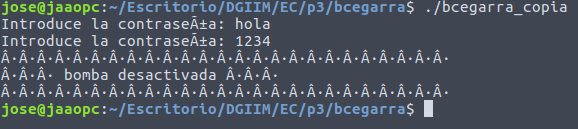
\includegraphics[scale=0.45]{capturas/bcegarra2.png} 
	\caption{Bomba Bcegarra modificada} \label{fig:figura25}
\end{figure}

\textbf{Por último, buscamos las claves de desactivación de la bomba.} He comenzado utilizando el comando \emph{strings}, que ha resultado ser muy práctica en esta bomba en particular. Al ejecutarlo con y sin \emph{-d} he visto que las strings \emph{password} y \emph{password2} eran nombres de variables, pues no aparecían en la ejecución con \emph{-d}, pero si en la otra.
Volviendo a gdb, podemos ver la salidas de \emph{print password} y \emph{print password2} en la foto de abajo. Al introducirlas, la bomba ha explotado. Tras utilizar de nuevo el comando \emph{strings} sobre la bomba y mirar la segunda contraseña, se me ha ocurrido que podía estar escrita al revés (ya que se lee \emph{marinabs} de esta forma, lo que tiene mucho más sentido). Efectivamente, al introducir esta nueva contraseña, la bomba ha quedado desactivada.
Ya tenemos las contraseñas: \textbf{DIP} y \textbf{marinasb}. \\


\begin{figure}[H] 
	\centering
	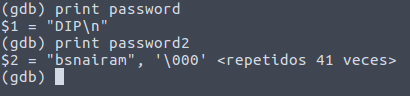
\includegraphics[scale=0.45]{capturas/bcegarraContras.png} 
	\caption{Bomba Bcegarra - contraseñas} \label{fig:figura25}
\end{figure}

\begin{figure}[H] 
	\centering
	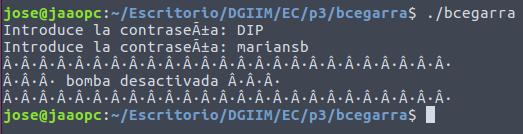
\includegraphics[scale=0.45]{capturas/bcegarra3.png} 
	\caption{Bomba Bcegarra resuelta} \label{fig:figura25}
\end{figure}

\title{\large{\textbf{\underline{Mi bomba: Eurus}}}} \\

El programa que he creado no difiere mucho de la bomba inicial. La mayor dificultad reside en encontrar el codigo, pues hacer que la bomba no se explote al ejecutarla o modificarla para que nunca lo haga es realmente sencillo. \\

Para el calcular si el código (al que llamaremos A) es correcto, Eurus utiliza 4 valores y un AND:
\begin{itemize}
	\item $B = 1119299126 = 2\cdot11^{3}\cdot61^{2}\cdot113$. 
	\item $C = 188495978 = 2\cdot11^{2}\cdot61\cdot113^{2}$.
	\item $D = 7381 = 11^{2}\cdot61$.
	\item $E = 68931 = 61\cdot113$.
	\item Máscara AND: $(A$ \& $0x1) == 0$.
\end{itemize}

Para que el código sea válida se ha de cumplir que A divida a B y a C (resto nulo), y que tanto C como D dividan a A (resto nulo). Para ello, A tiene que tener en su descomposición en primos a todos los primos que aparecen en las descomposiciones de D y E (pues al dividir estos a A, el resto ha de ser nulo). A su vez, la descomposicion factorial de A no podrá tener ningún número que no aparezca en las descomposiciones de tanto B como C, por el mismo razonamiento que para D y E. Además, para pasar la condición impuesta por la máscara AND, A tendrá que ser par (su último bit es 0). \\

El único número que cumple estas condiciones es $\textbf{A = 1668106} = 2\cdot11^{2}\cdot61\cdot113$. Para calcular si el número introducido es correcto, Eurus llama a una función, \emph{code}.\\

En cuanto a la contraseña, esta está definida en el código y es bastante sencillo encontrarla. Sin embargo, se la hace una pequeña modificación antes de compararla a la introducida: de \emph{miss me?} a \emph{miss\&me?}. Es sencillo apreciar este cambio en el código ensamblador. Procedo ahora a la desactivación de la bomba. \\

Por último quedan la pista el tiempo. El tiempo para introducir la primera contraseña es de 7 segundos. Sin embargo, la segunda contraseña la tenemos que introducir en \textbf{al menos 7 segundos}. Es decir, si el tiempo es inferior, la bomba explotará. Por otro lado está la pista, a la unicamente podemos acceder modificando el código en hexadecimal y haciendo que el último salto vaya a dicha posición (el del breakpoint 4). O bien, podemos descubrirla a traves del comando \emph{"strings"}. \\

\textbf{En primer lugar, ejecutaremos la bomba sin que esta explote.} Repetimos el proceso de rigor, ejecutamos con gdb evitando las llamadas a la funcion \emph{"boom"} modificando los valores de los registros: 

\begin{itemize}
	\item Breakpoint 1 - 0x80487eb - set \$eax = 0
	\item Breakpoint 2 - 0x804880f - set \$eax = 0
	\item Breakpoint 3 - 0x8048858 - set \$eax = 0
	\item Breakpoint 4 - 0x804887d - set \$eax = 7
\end{itemize}

\begin{figure}[H] 
	\centering
	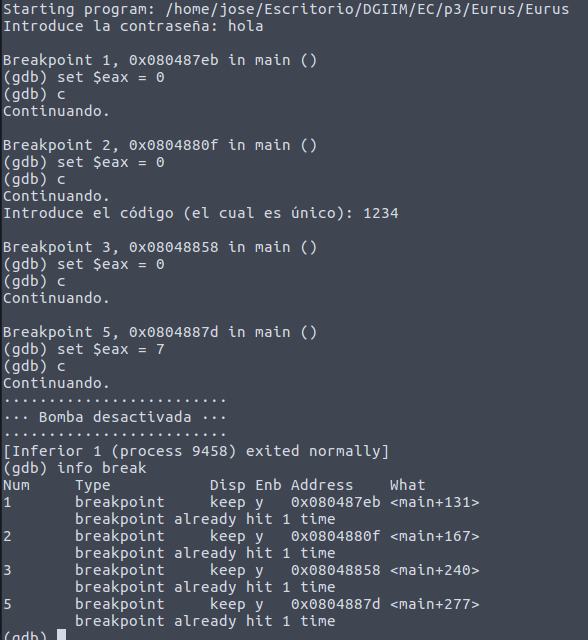
\includegraphics[scale=0.45]{capturas/Eurus1.png} 
	\caption{Eurus - gdb} \label{fig:figura25}
\end{figure}

\textbf{A continuación, modificamos la bomba para que nunca explote.} Para ello modificamos los 4 saltos del apartado anterior para que sean incondicionales, como hemos hecho en el resto de bombas. \\

\begin{figure}[H] 
	\centering
	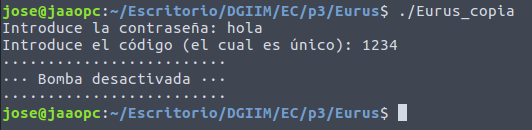
\includegraphics[scale=0.45]{capturas/Eurus2.png} 
	\caption{Eurus modificada} \label{fig:figura25}
\end{figure}

\textbf{Por último, buscamos las claves de desactivación de la bomba.} Ejecutando un rápido \emph{"strings -d bomba"} vemos que la única string que podría ser la contraseña es \emph{"miss me?"}. Al probar la contraseña vemos que la bomba explota. Con un rápido vistazo al objdump encontramos la siguiente línea: \\

 80487a1: $\quad$ c6 05 44 a0 04 08 26 $\quad$ movb $\quad$ \$0x26,0x804a044 \\

Buscando en una tabla 	ASCII descubrimos que el valor 0x26 = '\&'. Siendo la posición 0x804a044 el quinto elemento de la contraseña, el espacio en blanco, basta sustituirlo para caer en la cuenta de que la contraseña final es \textbf{miss\&me?}. \\

De hecho, con ejecutar gdb hasta justo antes de la llamada al \emph{strcmp} y hacer entonces el volcador de memoria mediante \emph{x/20cb 0x$<$dirección$>$} veríamos la contraseña modificada. \\

En cuanto al código, es sencillo darse cuenta de que si la función \emph{code} devuelve un 1 (almacenado en \%eax), la bomba explotará. Observando esta función paso por paso nos damos cuenta de que condiciones ha de cumplir la clave para que \emph{code} no devuelva 1, y así la bomba no explote. Aunque no obtendremos la clave como tal, estas condiciones (junto con una calculadora de descomposiciones en primos de internet) deberían bastarnos para poder obtener la clave final, no sin cierto esfuerzo. El proceso está explicado más detallado más arriba. \\

Finalmente obtendremos ambas contraseñas: \textbf{miss\&me?} y \textbf{1668106}. No olvidemos que para que la bomba no explote, hemos de esperar 7 segundos para introducir el código. \\   

\begin{figure}[H] 
	\centering
	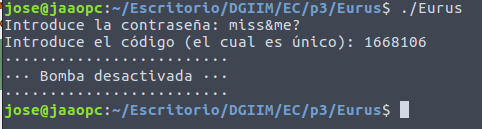
\includegraphics[scale=0.45]{capturas/Eurus3.png} 
	\caption{Eurus resuelta} \label{fig:figura25}
\end{figure}

\title{\large{\textbf{\underline{Conclusión final}}}} \\

La verdad es que he disfrutado mucho haciendo esta práctica. Una vez cogí cierto ritmo, se me ha hecho rápido y sencillo desactivar las bombas dedicándolos concentración. Me hubiese gustado que esta práctica estuviese fechada en otra época, ya que no le he dedicado ni la mitad del tiempo que me habría gustado, con los exámenes tan pegados. Respecto a mi bomba, después de los intentos, algunos frustados, por parte de mis compañeros, creo que quizás sea demasiado complicada. Añadí entonces la pista como ligera ayuda. \\
\end{document}